\documentclass[conference]{IEEEtran}
\usepackage{pifont}
\usepackage{times,amsmath,color,tabularx,caption,
amssymb,graphicx,epsfig,cite,psfrag,subfigure,algorithm,multirow,cases,balance}
\newtheorem{claim}{Claim}
\newtheorem{guess}{Conjecture}
\newtheorem{definition}{Definition}
\newtheorem{fact}{Fact}
\newtheorem{assumption}{Assumption}
\newtheorem{theorem}{\underline{Theorem}}
\newtheorem{lemma}{\underline{Lemma}}
\newtheorem{ctheorem}{Corrected Theorem}
\newtheorem{corollary}{\underline{Corollary}}
\newtheorem{proposition}{Proposition}
\newtheorem{example}{\underline{Example}}
\newtheorem{remark}{\underline{Remark}}
\newtheorem{problem}{\underline{Problem}}
\def\Ei{\mathop\mathrm{Ei}}
\def\E{\mathop\mathrm{E}}
\def\tr{\mathop\mathrm{tr}}
\newcounter{mytempeqncnt}
%\IEEEoverridecommandlockouts

\begin{document}

\title{Literature Survey -- Draft II \\ Unsupervised Feature Learning and Deep Learning}
\author{Jiachen Li (Andrew ID: jiachenl)\\%
Language Technologies Institute, Carnegie Mellon University, Pittsburgh, PA, 15213, USA\\
Email: jiachenl@cs.cmu.edu
}

%\thanks{This work was supported...}




\maketitle %\thispagestyle{empty}




\begin{abstract}
Machine Learning has proven to be a big success in many areas of artificial intelligence. However, the success of these algorithms highly depends on how good the features are represented. A good representation of feature is surely
to enhance the performance of machine learning algorithms, while a poor representation may not only severely limit the performance
but even ruin the results. In this literature survey, I will do a review about the field of unsupervised feature learning and has an emphasis on learning feature representation through deep learning architecture. This survey will start with the problems about unsupervised feature learning. After that, it will introduce some typical algorithms in unsupervised feature learning and deep learning. Moreover, it will provide a few successful examples by using unsupervised feature learning. Finally, the conclusion as well as the potential feature works will be included at last.

\end{abstract}

\section{Introduction}

The performance of machine learning algorithms, especially the simpler ones  highly depends on how good the features are represented \cite{review}. For this reason, much of the effort in deploying machine learning algorithms in real problems has been paid to the process of feature extraction. During the past decades, feature extraction does play an very important role in the development of machine learning, where the machine learning research communities have spent a lot of efforts on manually designing or creating new features through domain knowledge and some other special techniques. For example, the MFCC feature in speech recognition and the HoG feature in computer vision. However, though these features may often contain the deep insights about a specific problem or some incredibly clever ideas, we cannot avoid the fact that the way to create such features costs a lot of human labor and the feature representation derived often cannot be extended to other problems, especially when we encounter into them in a new filed. So the problem comes up that is there any way to learn the feature representation automatically and is there any way to do better than the manually created features. Fortunately, the answer is yes to both of the questions, and the way is unsupervised feature learning.

\subsection{What Is Unsupervised Feature Learning?}

\begin{figure}[t]
\centering
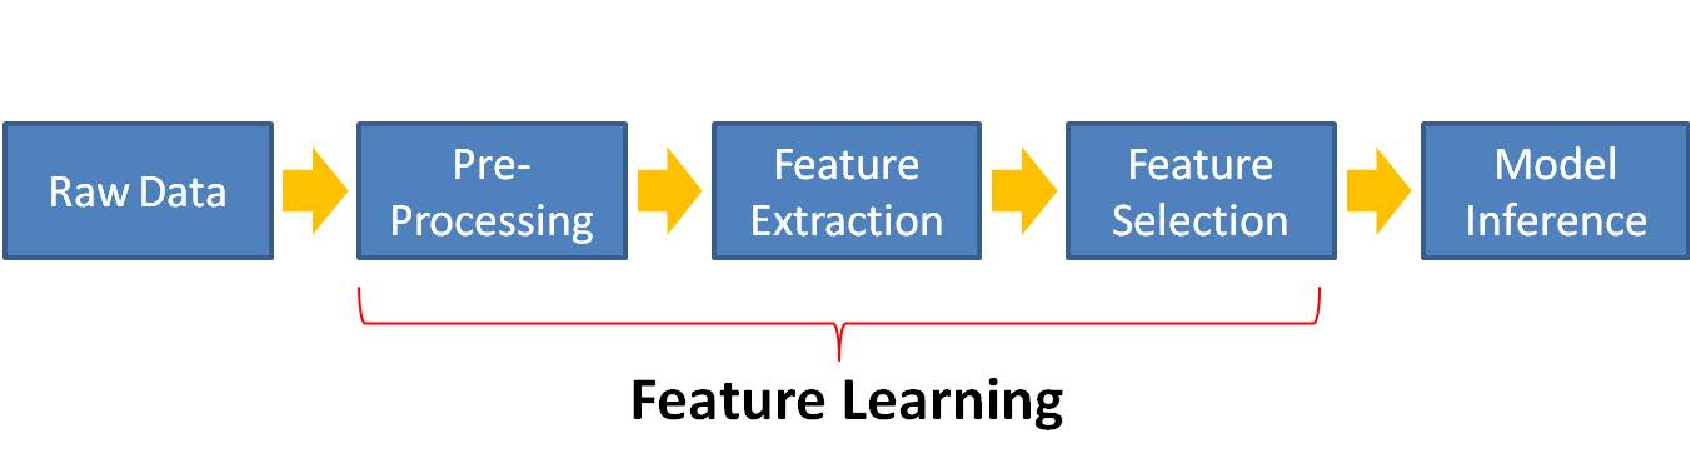
\includegraphics[width=85mm]{feature_learning.pdf}
\caption{The general framework of machine learning task.}
\label{fig:ml_task}
\end{figure}

To answer the question that what is unsupervised feature learning, let's start by looking at the general framework of solving a machine learning task. To solve a machine learning problem, as shown in Fig. \ref{fig:ml_task}, we should first do pre-precessing for the raw data, such as the data cleaning, and then perform feature extraction on the data processed. After that, we apply our feature extraction algorithm to extract the useful features, do feature selection on these extracted features and then use them for training models. With a well trained model, we can finally approach to our goals like classification or regression.

In the above framework, the procedures of pre-processing, feature extraction and feature selection together can be summarized as the ``feature learning''.
Moreover, the term ``unsupervised'' means that we can this kind of feature learning procedures to be performed without our supervision (knowledge) or even without any of our help.

\subsection{Differences with other Machine Learning Tasks}



One of the major differences that distinguishes unsupervised feature learning from other machine learning tasks such as classification is the ultimate goal during the training phase. To be specific, in the case of classification, the typical objective is to minimize the classification errors on the training set, so that we can learn a classifier or predictor for future use. However, in the unsupervised feature learning, the goal changes to learn the representation of feature automatically, which means the algorithms will make their own decisions on what is going to learn. Therefore, the features learned will no long be specified by human. And this is also totally different from the paradigm of feature engineering where people design by hands on what to learn.

\subsection{Types of Unsupervised Feature Learning}

There are two common unsupervised feature learning settings, depending on what type of unlabeled data you have. The more general and powerful setting is the self-taught learning setting, which does not assume that your unlabeled data $\mathbf{x}_u$ has to be drawn from the same distribution as your labeled data $\mathbf{x}_l$ \cite{self_taught}. The more restrictive setting where the unlabeled data comes from exactly the same distribution as the labeled data is sometimes called the semi-supervised learning setting. This distinctions is best explained with an example, which we now give.

\subsection{Organization of this Review}

The reminder of this literature survey is organized as follows: Section II defines the feature learning problem and the learning strategy. Section III introduces the models and algorithms for feature learning. A few successful examples are then given in section IV, and the conclusions and potential future works are drawn in section V.

\section{Feature Learning Problem and Learning Strategy}

Suppose that we have a large set labelled or unlabelled data as input, i.e., $$\mathcal{S}=\{\mathbf{x}^{(1)},\mathbf{x}^{(2)},\mathbf{x}^{(3)},\ldots\}, \ \mathbf{x}^{(i)}\in\mathcal{R}^n.$$
Then what the feature learning wants to do is to train a model
\begin{equation}
\Psi(\mathbf{x}):\mathcal{X} \rightarrow \mathcal{F},
\end{equation}
which can extract rich and high-level structures (as the high-level features) from the origin input space ($\mathcal{X}$) to the feature space ($\mathcal{F}$). So the problem is how can we let the machine automatically learn such kinds of feature?

The answer to this question is to learn the feature by levels or layers, which means that to learn the final representation of the data, we may start by learning some lower level representation of the data (low level feature). Next, with the combination of these low level features, we can then further learn some higher level representation of the data (high level feature). So, if we continue this process, then we can finally learn a good representation of the data.




This layer-based learning strategy is first inspired by the study of our vision system, where the researchers reveal that the mammal brain is organized in a deep architecture \cite{visual}
with a given input percept represented at multiple levels of abstraction,
each level corresponding to a different area of cortex. Humans
often describe such concepts in hierarchical ways, with multiple levels
of abstraction. The brain also appears to process information through
multiple stages of transformation and representation. This is particularly
clear in the primate visual system \cite{visual}, with its sequence of
processing stages: detection of edges, primitive shapes, and moving up
to gradually more complex visual shapes.
For example, as shown in Fig. \ref{fig:feat_level}, if our visual system want to learn some representations of different faces with the pixel input from eyes, it may first try to learn the representation of edges (low level feature) from the input pixels. Then, with the combination of different edges, it can further learn the representation of different object parts on our faces, such as noises, mouses and so on (medium level feature). Finally, with the combination of these different object parts, we can learn to form different faces, which can be regarded as the high level feature.

\begin{figure}[t]
\centering
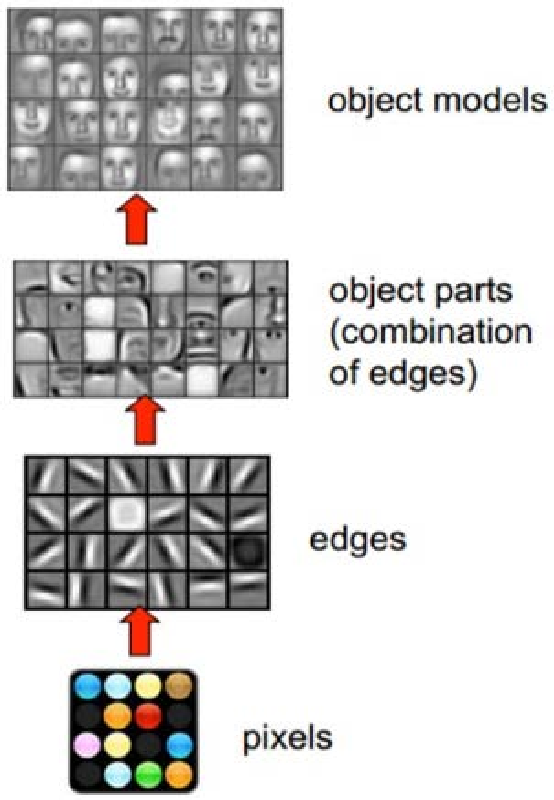
\includegraphics[width=60mm]{feat_level.pdf}
\caption{An illustration of learning feature representation by levels \cite{face}.}
\label{fig:feat_level}
\end{figure}

\begin{remark}
The layer-based learning strategy is reasonable as it is consistent with the way human used to learn things. For example, if want learn the meaning of a paragraph, we may first want to learn the meaning of each single word.
Next, with the meaning of each word and their combination in the sentences, we can learn the meaning of each sentence. Then with the meaningful of each sentence, it is much more easier for us to learn the meaning of the whole paragraph.
\end{remark}

\section{Feature Learning: Models and Algorithms}

Deep neural networks or deep learning is a learning model where the deep architecture is applied to perform the intellectual learning like learning to represent feature. This ability, together with the efficient learning algorithms that can ensure this ability, point out a new direction in the task of unsupervised feature learning, i.e., learning deep representation of the feature. In this section, I will review the work related to the deep learning in recent years, with a focus on some typical learning architectures and learning algorithms. The application of it in unsupervised feature learning will be discussed in the next section.


\subsection{Background and Motivation}

Deep learning methods aim at learning feature hierarchies with features from higher levels formed by the composition of the features from lower levels. Learning features at multiple levels of abstraction allows a system to learn complex functions mapping the input data to output feature, which is especially important for higher-level abstractions where humans often don't know how to specify the explicit feature extraction algorithms.

Deep architecture refers to the model architecture that can learn multiple levels non-linear transformation. So that the depth of architecture refers to the number of levels of composition of non-linear transformation in the function learned. Most current popular learning algorithms such as Logistic Regression (no hidden layer), Support Vector Machine (one hidden layer) and Boosting (one hidden layer) are using the shallow architectures. However, inspired by the architectural depth of the brain, neural network researchers had wanted for decades to train deep multi-layer neural networks. Unfortunately, no successful attempts were reported: researchers reported positive experimental results with typically two or three levels (i.e., one or two hidden layers), but training deeper networks consistently yielded poorer results.

In 2006, a breakthrough in feature learning and deep learning was initiated by Geoff Hinton, he introduced Deep Belief Networks (DBNs) together with a learning algorithm\cite{Hinton} and was quickly followed up in the same year by many others. The central idea, referred to as \textit{greedy layerwise unsupervised pre-training}, was to learn a hierarchy of features one level at a time, using unsupervised feature learning to learn a new transformation at each level to be composed with the previously learned transformations.

Since 2006, deep networks for feature learning has been applied widely with success not only in classification tasks, but also in regression, dimensionality reduction, speech recognition, object segmentation, information retrieval, robotics, natural language processing and collaborative filtering\cite{AI}.


\subsection{Deep Belief Networks (DBNs)}

There are several types of deep neural networks such as deep belief networks (DBNs) and convolutional neural networks (CNNs). Among them DBNs is not only one of the milestones in the realm of deep learning, but also very capable for unsupervised feature learning. Therefore, in this part, I'll mainly focus on DBNs, and cover its details in learning feature representation.


DBNs is a hybrid model consisting of two parts. As shown in Fig. \ref{fig:dbn}, the top two levels are undirected graph model which form the associative memory, the remaining layers are directed graph model which is actually a stacked Restricted Boltzmann Machines (RBM). Different from the CNNs, DBNs is a stochastically learning architecture whose object
function depends on the learning purpose. Generally speaking, DBNs can be trained as a discriminative model or a generative model. In Fig. \ref{fig:dbn} , the discriminative model is a ``bottoms-up'' approach (red arrow), trying to
learn the detection weights via optimizing a posterior probability $P(L|O)$, where $L$ indicates the label while $O$ is the observation; the generative model is a ``top-down'' approach (green arrow), trying to learn the generative weights via optimizing a joint probability $P(L,O)$.

%The details of the learning strategies will be discussed in the next part of this section.

Another description of DBNs is from Hinton et al. \cite{Hinton}, where they showed that Restricted Boltzmann Machine (RBMs) can be stacked and trained in a greedy manner to form so-called DBNs. They model the joint distribution between observed vector $\mathbf{x}$ and the $l$ hidden layers as:
\begin{equation}
P(\mathbf{x},h^1,\ldots,h_l)=\Big(\prod_{k=1}^{l-2} P(h^k|h^{k+1})\Big)
P(h^{l-1},h^l),
\end{equation}
where $x=h^0,\ P(h^{k-1}|h^k)$ is a conditional distribution for the visible units conditioned on the hidden units of the RBM at level $k$, and $P(h^{l-1},h^l)$ is the visible-hidden joint distribution in the top-level RBM.


The greatest advantage of DBNs is its capability of learning multi-level representation of feature, which is achieved through a layer-wise training strategy where the higher-level features are learned based on the features produced by the previous layers. Therefore, the higher-level features are believed to be more complicated and can better represent the information extracted from the structure of input data. Furthermore, we can also prove that after we adding another layer of features, we improve a variational lower bound on the log probability of the training data \cite{Hinton}.

\begin{figure}[t]
\centering
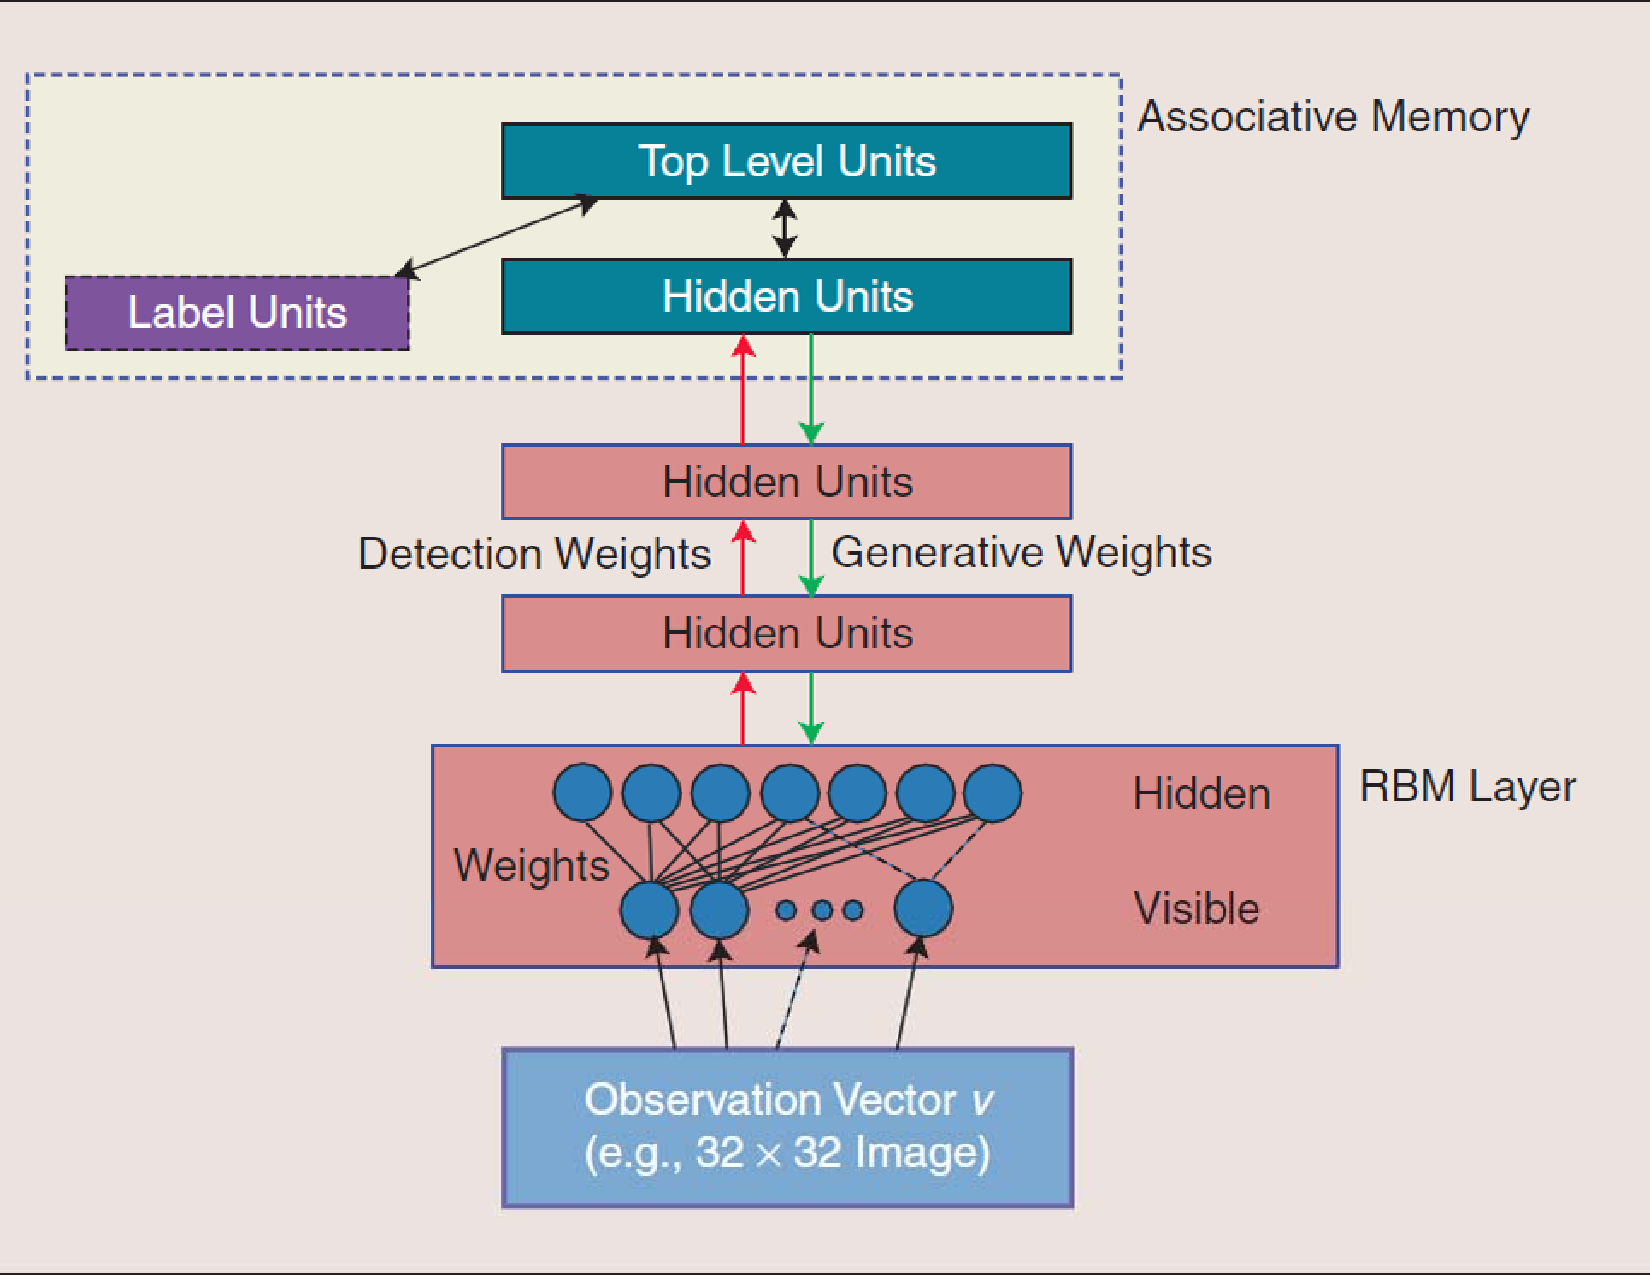
\includegraphics[width=80mm]{dbn.pdf}
\caption{Illustration of deep belief networks\cite{new_frontier}.}
\label{fig:dbn}
\end{figure}

\subsection{Challenge of Training Deep Neural Networks}

After having motivated the need for deep architecture and the advantages of deep belief networks, now we turn to the difficult problem of training them.
Experimental evidence suggests that training deep architectures is more difficult than training shallow architectures\cite{AI}.

One of the biggest problems when applying traditional gradient-based training for deep neural networks is that the random initialized multi-layer neural networks gets stuck in ``apparent local minima or plateaus'', and it becomes more difficult to obtain good generalization as the architecture gets deeperp. When starting from random initialization, the solutions obtained with deeper neural networks perform even worse than the solutions obtained for networks with 1 or 2 hidden layers. This happens even though $k+1$-layer nets can easily represent what a $k$-layer net can represent, but the converse is not true.

So, to take advantages of deep architectures, we need a new way to train these models.

\subsection{Train DBNs for Feature Learning}

In this part, I'll discuss the training strategy in deep learning architecture. We will focus on the training of DBNs since it is not only one of the typical models in deep learning, but also very suitable for the feature learning.

Generally speaking, the training process of DBNs usually consists of two parts, one is the pre-training, the other is fine-tuning.

\subsubsection{Pre-Training}

In the part of pre-training, one of the popular and easy-implement choice is the greedy layer-wise unsupervised pre-training \cite{greedy}. The key idea of this approach is to learn a hierarchy of features one level at a time, using unsupervised feature learning to learn a new transformation at each level to be composed with the previously learned transformations. During the learning phase, each iteration of unsupervised feature learning adds a new layer of weights to the whole deep neural network. Finally the set of layers could be combined to transform the input data into a set of learned high-level features through a series of non-linear transformation.



\begin{remark}
If we regard the layer-wise pre-training as learning the representation of feature from the input data, then the whole pre-training process can be considered as learning the representation of the original data layer by layer. So, intuitively, learning the feature representation of data can be performed though training the deep neural networks.
\end{remark}

\subsubsection{Fine-tuning}

After pre-training, the weights between each adjacent layers can somehow reflect the relationship with the data themselves. Furthermore, in order to ensure a better performance, we use fine-tuning to adjust these weights according to different model types we assume.

For the discriminative model, back-propagation algorithm is used to adjust the detection weights by supervised learning using the labeled
data. There��s nothing new about the Back-propagation, the only thing we should pay attention to is that we should carefully set the learning rate since a too-big value will change the pre-trained weights a lot. However, we should also notice that there is a trade-off as a too-small value will lead to a slow tuning procedure.

For the generative model, a Wake-Sleep algorithm is used to tune the generative weights. Wake is a bottom-up procedure, which uses the learning RBM approach to approximate the joint distribution showed in the following term
\begin{align}
&P(v,h_1,h_2,\ldots h_n) \nonumber \\ = &P(h_1|v)P(h_2|h_1,v)\cdots
P(h_n|h_{n-1},\ldots,h_1,v).
\end{align}
Since detection weights are learned in this procedure, we can sample all the $v,h1,h2,\ldots,hn$. Then, these sampled data is used to tune the generative weights, which is to maximize term
\begin{align}
&P(v,h_1,h_2,\ldots h_n)\nonumber \\ =& P(h_{n-1}|h_n)P(h_{n-2}|h_{n-1},h_n)\cdots P(v|h_n,\ldots h_1).
\end{align}
Since all units are known, it is easy to solve this maximization problem.
Therefore, wake stage is a ��bottom-up�� procedure tuning the generative weights. Tuning only once is not enough, so we also need the sleep stage which is similar to wake, but it is ��top-down�� approach and tunes the detection weights. We iteratively call the wake and sleep stages until the convergence is reached, which indicates the end of fine-tuning.


\section{Applications of Unsupervised Feature Learning}

In the previous sections,p I have shown that why should we study feature learning, what strategy should we use in feature learning and what model should we apply in unsupervised feature learning. In this section, I'll refer to some successful real world applications to show the powerful usage of unsupervised feature learning as well as how the machine learning tasks benefit from the unsupervised feature learning.


\subsection{Unsupervised Feature Learning in Speech Recognition}

\begin{figure}[t]
\centering
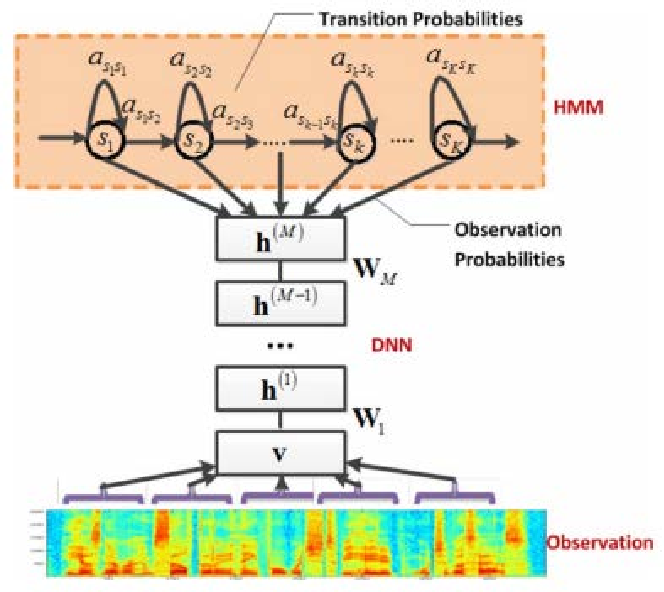
\includegraphics[width=80mm]{cd-dnn-hmm.pdf}
\caption{Diagram of the hybrid architecture in speech recognition employing a deep neural network \cite{cd-dnn-hmm}.}
\label{fig:cd-dnn-hmm}
\end{figure}

Since the early 90��s, artificial neural networks (ANNs) have
been used to model the state emission probabilities of HMM
speech recognizers. While traditional Gaussian mixture
model (GMM-HMMs) models context dependency through tied
context-dependent states, ANN-HMMs were never used to do so directly.
Instead, neural networks were often factorized, e.g. into a monophone
and a context-dependent part, or hierarchically decomposed. It has been commonly assumed that hundreds or thousands of triphone states were just too many to be accurately modeled or trained within a neural network.

Only recently did Yu et al. discover
that doing so is not only feasible but works very well \cite{cd-dnn-hmm}.
As shown in Fig. \ref{fig:cd-dnn-hmm}, the Context-dependent Deep-Neural-Network HMMs (CD-DNN-
HMMs) applies deep belief network as a feature learner to extract more powerful, more robust features and map them into different HMMs states. Utilizing Hinton's DBN pre-training (unsupervised feature learning) procedure, this model leads to a very promising results with a $22~33\%$ decrease in word error rate as shown in Table. I.


\begin{table*}[ht]\label{Tab:1}
\captionsetup{font={small}}
\caption{Standard GMM-HMM vs. CD-DNN-HMM for single-pass speaker-independent recognition on five speech-to-text test sets. Also shown are our group's best-ever GMM-HMM result for three of the test sets. Transcription word-error rates are given in $\%$.}
\centering
\begin{tabular}{|c|c|c|c|c|c|c|c|}
\hline
acoustic model \& training & recognition mode & \multicolumn{2}{c|}{RT03S}  & Hub5'00 & \multicolumn{2}{c|}{voicemails} & teleconf \\
& & FSH & SW & SWB & MS& LDC &  \\
\hline\hline

GMM 40-mix, ML, SWB 309h & single-pass SI & 30.2 & 40.9 & 26.5 & 45.0 & 33.5 & 35.2 \\
GMM 40-mix, BMMI, SWB 309h & single-pass SI & 27.4&37.6 &23.6 &42.4 &30.8 &33.9 \\
CD-DNN 7 layers x 2048, SWB 309h & single-pass SI & 18.5&27.5 &16.1 &32.9 &22.9 &24.4 \\
(rel. change GMM BMMI��CD-DNN) & &(-33\%) &(-27\%) &(-32\%) &(-22\%) &(-26\%) &(-28\%) \\
\hline\hline
GMM 72-mix, BMMI, Fisher 2000h & multi-pass adaptive &18.6 &25.2 &17.1 & & & \\
\hline
\end{tabular}
\end{table*}

\subsection{Unsupervised Feature Learning in Information Retrieval}

TODO:...

\section{Conclusions}

Let machine learn the feature by themselves is fascinating as well as challenging, while the unsupervised feature learning gives us a chance to make it come true. In this literature survey, a broad overview of unsupervised feature learning on different aspects is given by answering the following questions, such as why we study unsupervised feature learning and deep learning, how to let machine learn feature representation by themselves, which model should we use for unsupervised feature learning and how can machine learning tasks benefit from unsupervised feature learning and deep learning. I not only show how the deep learning can be used for unsupervised feature learning, but also give an intuition about why it works. At last, many real world applications has been presented to show that unsupervised feature learning can be really helpful.

\section*{Acknowledgement}
I would like to thank Prof. Eric Nyberg for his advice on my presentation and his constructive suggestions on this literature survey.


%\balance
\begin{thebibliography}{99}

\bibitem{review} Y. Bengio, A. Courville, and P. Vincent, ``Representation Learning: A Review and New Perspectives,'' in \textit{IEEE Trans. Pattern Analysis and Machine Intelligence}, vol. 35, no. 8, pp. 1798--1828, 2013.

\bibitem{self_taught} R. Raina, A. Battle, H. Lee, B. Packer, and A. Y. Ng. ``Self-taught learning: Transfer learning from unlabeled data,'' \textit{Proc. Int'l Conf. Machine Learning}, 2007.

\bibitem{face} H. Lee, R. Grosse, R. Ranganath, and A. Y. Ng, ``Unsupervised Learning of Hierarchical Representations with Convolutional Deep Belief Networks'' \textit{Communications of the ACM}, vol. 54, no. 10, pp. 95--p103, 2011.


\bibitem{new_frontier} I. Arel, D. C. Rose, and T. P. Karnowski, ``Research frontier: Deep machine learning-a new frontier in artificial intelligence research,'' \textit{Comp. Intell. Mag.}, vol. 5, no. 4, pp. 13--18, Nov. 2010.

\bibitem{Hinton} G. E. Hinton, S. Osindero, and Y. Teh, ``A fast learning algorithm for deep belief nets,'' \textit{Neural Computation}, 18, pp 1527--1554, 2006.

\bibitem{visual} T. Serre, G. Kreiman, M. Kouh, C. Cadieu, U. Knoblich, and T. Poggio, ``A quantitative theory of immediate visual recognition,'' \textit{Progress in Brain Research, Computational Neuroscience: Theoretical Insights into Brain Function}, vol. 165, pp. 33--56, 2007.

\bibitem{AI} Y. Bengio, ``Learning deep architectures for AI,'' \textit{Foundations and Trends in Machine Learning}, vol 2, pp 1--127. Also published as a book. Now Publisher, 2009.

\bibitem{greedy}  Y. Bengio, P. Lamblin, D. Popovici, and H. Larochelle, ``Greedy Layer-Wise Training of Deep Networks,'' \textit{Proc. Neural Information and Processing Systems}, 2006.

\bibitem{cd-dnn-hmm} G. E. Dahl, D. Yu, L. Deng, and A. Acero. ``Context-Dependent Pre-Trained Deep Neural Networks for Large-Vocabulary Speech Recognition,'' \textit{IEEE Transactions on Audio, Speech and Language Processing}, vol. 20, no. 1, Jan. 2012.


\bibitem{Frank} F. Seide, G. Li, and D. Yu, ``Conversational Speech Transcription Using Context-Dependent Deep Neural Networks'' \textit{Interspeech}, 2011.



\bibitem{dAE} P. Vincent, H. Larochelle, Y. Bengio, and P. Manzagol. ``Extracting and composing robust features with denoising autoencoders,'' \textit{Proc. Int'l Conf. Machine Learning}, 2008.
\bibitem{CNN} H. Lee, R. Grosse, R. Ranganath, and A. Y. Ng, ``Convolutional deep belief networks for scalable unsupervised learning of hierarchical representations,'' \textit{Proc. Int'l Conf. Machine Learning}, 2009.
\bibitem{why} D. Erhan, Y. Bengio, A. Courville, P. Manzagol, P. Vincent, and S. Bengio, ``Why Does Unsupervised Pre-training Help Deep Learning?'' \textit{Journal of Machine Learning Research}, 2010.
%\bibitem{kmeans} A. Coates and A. Y. Ng, ``Learning Feature Representations with K-means,'' \textit{Neural Networks: Tricks of the Trade}, Springer LNCS, 2012.

\bibitem{Yudong} L. Deng and D. Yu ``DEEP LEARNING: Methods and Applications,'' NOW Publishers, 2014.



\end{thebibliography}

\section{SUMMARY}

This is the second draft of my literature survey, I mainly finished: \\
1. Main contents in all sections \\
2. Added more backgrounds in deep learning (as required in presentation) \\
3. Added first example in speech recognition. \\

For the next final version, I'm planning to finish: \\
1. Add more application examples \\
2. Include more theoretical analysis. \\
3. Add more figures to illustrate the key ideas. \\
4. Polish the language usage.

%\begin{table}[t]\label{Tab:1}
%\centering \caption{$Required\ Interference\ Protection\
%Ratios$}
%\begin{tabular}{|c|c|c|}
%\hline
%Type of service & Channel & Interference \\
%& Offset & Protection D/U \\
%& & Ratio(dB) \\
%\hline
%Analog TV & Lower Adjacent & -14 \\
%\cline{2-3}
%& Co-channel & 34 \\
%\cline{2-3}
%& Upper Adjacent & -17 \\
%\hline
%Digital TV & Lower Adjacent & -28 \\
%\cline{2-3}
%& Co-channel & 23 \\
%\cline{2-3}
%& Upper Adjacent & -26 \\
%\hline
%\end{tabular}
%\end{table}








\end{document}
